\documentclass[runningheads]{llncs}

\usepackage{amssymb}
\usepackage{amsmath}
\usepackage{float}
%% The amsthm package provides extended theorem environments

% \usepackage{amsthm}
% AM commented out because it clashes with proof, etc

%% The lineno packages adds line numbers. Start line numbering with
%% \begin{linenumbers}, end it with \end{linenumbers}. Or switch it on
%% for the whole article with \linenumbers.
\usepackage{lineno}

%% Use package enumitem to align enumeration and itemization
\usepackage{enumitem}
\usepackage{listings}
%\usepackage{courier}           % for the courier font (optional)
\usepackage{multicol}          % for two equations side by side
\usepackage[justification=centering]{caption}
\usepackage[dvipsnames]{xcolor}
\usepackage{stmaryrd}
\usepackage{hyperref}
%\usepackage{cleveref}
\usepackage{hieroglf}
\usepackage{scalerel}
\usepackage{tikz}
\usepackage{pgfplots}
\usepackage[export]{adjustbox} % for subfigures
\usepackage{semantic}          % for mathlig


\hypersetup{ % play with these to change the look of hyperlinks
	colorlinks=true,
	linkcolor=black,
	filecolor=magenta,
	urlcolor=blue,
	citecolor=black
}

\newcommand{\coq}{\scalebox{.6}{\textpmhg{\Ha}}}
\newcommand{\p}[1]{\ensuremath{\mathsf{#1}}} % predicate font
\newcommand{\m}[1]{\ensuremath{\mathit{#1}}} % math font
\newcommand{\braces}[1]{\left\{\begin{array}{l@{}} #1 \end{array}\right\}}
\let\ramify\lightning
\newcommand{\sz}{\texttt{SIZE}}
\newcommand{\ifty}{\texttt{INF}}
\newcommand{\defeq}{\mathbin{\stackrel{\Delta}{=}}}
\newcommand{\bigO}{\text{O}}
\usetikzlibrary{shadows}
\usetikzlibrary{arrows.meta, positioning, decorations.pathmorphing, fit, matrix}
\mathlig{/|}{\mathbin{\wedge}} % additive conjunction


% required by LNCS
\renewcommand\UrlFont{\color{blue}\rmfamily}

\colorlet{red}{red!80!black}
\colorlet{green}{green!50!black}

%% NEW COMMANDS =============================================

\lstdefinestyle{myStyle}{
	%	language=Coq,
	keywords={Inductive,Require,Import,Definition,Fixpoint,match,with,end,let,in,fix},
	basicstyle=\normalfont\footnotesize\tt,
	keywordstyle=\color{green}, % Blue clashes with the cyan links. Change if you want.
	stepnumber=1,
	tabsize=2,
	numbers=none,
	numberstyle=\tiny,
	numbersep=5pt,
	showspaces=false,
	escapechar=`,
	showstringspaces=false
}
%basicstyle=\fontsize{10}{11}\selectfont\ttfamily,

\lstdefinestyle{myTinyStyle}{
	%   language=Coq,
	basicstyle=\normalfont\fontsize{7.0}{7.3}\tt,
	keywordstyle=\color{green}, % Blue clashes with the cyan links. Change if you want.
	stepnumber=1,
	tabsize=2,
	numbers=none,
	numberstyle=\tiny,
	numbersep=5pt,
	showspaces=false,
	showstringspaces=false,
	language=C,
	morecomment=[l][{\color{OliveGreen}}]{//},
	sensitive=true,
	mathescape=true,
	showlines=true,
	escapechar=`,
	basicstyle=\footnotesize\ttfamily,
	keywordstyle=\color{blue}, numbers=left,
	numberstyle=\tiny, numbersep=5pt, boxpos=t
}

\lstset{style=myTinyStyle}
\makeatletter
\newlength{\@mli}
\newcommand{\mli}[1]{%
	\settowidth{\@mli}{\lstinline/#1/}
	\hspace{-.5ex}\begin{minipage}[t]{\@mli}\lstinline/#1/\end{minipage}}
\makeatother
\newcommand{\li}[1]{\ifmmode\mbox{\mli{#1}}\else\mbox{\lstinline/#1/}\fi}

\newcommand\hide[1]{}

\newenvironment{centermath}
{\begin{center}$\displaystyle}
	{$\end{center}}

\renewcommand{\note}[2][polish]{{\color{red} #2}{\marginpar{\tiny \color{blue} #1}}}
\renewcommand{\implies}{\Rightarrow}
\renewcommand{\iff}{\Leftrightarrow}

\title{A Machine-Checked C Implementation of Dijkstra's Shortest Path Algorithm}
\titlerunning{A Machine-Checked C Implementation of Dijkstra's Shortest Path Algorithm}
%optional, please use if title is longer than one line

\begin{document}

	\author{Anshuman Mohan\inst{1} \and 
	Wei Xiang Leow\inst{1} \and 
	Shengyi Wang\inst{2} \and 
	Aquinas Hobor\inst{1,3}}

	\authorrunning{A. Mohan et al.}
% First names are abbreviated in the running head.
% If there are more than two authors, 'et al.' is used.
	
	\institute{School of Computing, National University of Singapore \and
	Princeton University, USA \and
	Yale-NUS College, National University of Singapore}	
	
	\maketitle
	%\begin{frontmatter}
	
	%% Title, authors and addresses
	
	%% use the tnoteref command within \title for footnotes;
	%% use the tnotetext command for theassociated footnote;
	%% use the fnref command within \author or \address for footnotes;
	%% use the fntext command for theassociated footnote;
	%% use the corref command within \author for corresponding author footnotes;
	%% use the cortext command for theassociated footnote;
	%% use the ead command for the email address,
	%% and the form \ead[url] for the home page:
	
	%% \tnotetext[label1]{}
	%% \author{Name\corref{cor1}\fnref{label2}}
	%% \ead{email address}
	%% \ead[url]{home page}
	%% \fntext[label2]{}
	%% \cortext[cor1]{}
	%% \address{Address\fnref{label3}}
	%% \fntext[label3]{}
	
	%% use optional labels to link authors explicitly to addresses:
	%% \author[label1,label2]{}
	%% \address[label1]{}
	%% \address[label2]{}
	
	%\author{}
	
	%\address{}
	
	
	\begin{abstract}
		\vspace{-1.2em}
		We extend our research group's previous work on verifying C graph implementations
		with verified versions of Dijkstra's, Prim's and Kruskal's classical algorithms.
		We prove functional correctness of C implementations of these algorithms, and expand the previous graph library to reason about undirected graph properties and common spatial representations.
		
		In particular, we encounter and explain an overflow issue in Dijkstra’s algorithm. The precise bound in the relevant precondition is nontrivial: we show that the intuitive guess fails and provide a workable refinement. We also make an observation of Prim's algorithm that contradicts the common consensus that the basic algorithm cannot work on disconnected graphs - our implementation is able to compute minimum spanning forests without finding components first.
		
		This work fits into an ongoing exploration of verified graph-manipulating algorithms in a realistic setting.
		
		\keywords{Dijkstra's shortest-path \and Prim's algorithm \and Kruskal's algorithm \and minimum spanning trees \and verification \and CompCert \and VST}
	\end{abstract} %\and Coq 
	
	%\end{frontmatter}
	
	%% \linenumbers
	
	%% main text
	
	\section{Introduction}
	\label{sec:intro}
	Over the last fifteen years great strides have been made in automating verifications of programs that manipulate
tree-like data structures using separation logic 
\cite{berdine:smallfoot,chin:hipsleek,jacobs:verifast,chlipala:bedrock,bengtson:charge,appel:programlogics}.  Unfortunately, verifying programs that manipulate graph-like data structures (i.e. structures with \emph{intrinsic sharing}) has been more challenging.  Indeed, verifying such programs was formidable enough that a number of the early landmark results in separation logic devoted substantial effort to verify single examples such as Schorr-Waite~\cite{hongseok:phd} with pen and paper---avoiding the additional challenges inherent in mechanized reasoning.

In recent years, Hobor and Villard introduced the concept of \emph{ramification} as a kind of proof pattern or framework to verify graph-manipulating programs on pen and paper~\cite{hobor:ramification}.  The major focus of this paper is to develop methods to verify realistic graph programs in a mechanized context.  We do so by upgrading the theory of ramification and by developing a general and modular library for graph-related reasoning in separation logic.  We incorporate our approach into two sizeable separation logic-based verification tools: the Floyd system of the Verified Software Toolchain (VST)~\cite{appel:programlogics} and the HIP/SLEEK program verifier~\cite{chin:hipsleek}.  VST and HIP/SLEEK inhabit quite different points in the design space for verification tools, with VST primarily focused on heavily human-guided verifications with an emphasis on end-to-end machine-checked proofs, and HIP/SLEEK focusing on more automation.  Despite these differences, the vast majority of our Coq code base is shared between them,
giving us hope that our work will be applicable to other verification tools.

\marginpar{\color{magenta} computable mathgraphs, null, pregraphs Problem with ``later'' not being precise.}
The structure of our paper is as follows:
%\vspace{-0.25ex}
\begin{itemize}
\item[\S\ref{sec:orientation}] We verify a graph marking algorithm and explain why such algorithms are easier to verify using relations instead of functions.  We introduce \emph{localization blocks} as a new notation for ramification.  We upgrade Hobor and Villard's \infrulestyle{Ramify} rule to handle both modified program variables and existential quantifiers more gracefully.
\vspace{-0.1ex}
\item[\S\ref{sec:mathgraph}] We develop a general mechanization of mathematical graphs powerful enough to support realistic verification. %{\color{magenta} What else can we say here?}
\vspace{-0.1ex}
\item[\S\ref{sec:spacegraph}] We show that the standard Knaster-Tarski fixpoint~\cite{tarski:fixpoint} cannot define a usable separation logic graph predicate.  We propose a better definition for general spatial graphs that still enjoys a ``recursive'' fold/unfold.  We prove general theorems about spatial graphs in a way that can be utilized in multiple flavors of separation logic, such as the logics contained in VST and HIP/SLEEK.
\vspace{-0.1ex}
\item[\S\ref{vst}] We explain how we integrated ramification into VST by developing two new Floyd tactics, \li{localize} and \li{unlocalize}.  We discuss other examples we have verified, including spanning tree and DAG copy.
\vspace{-0.1ex}
\item[\S\ref{sec:hipsleek}] We explain how we modified HIP/SLEEK to introduce ramifications when programs modify data structures with intrinsic sharing and to automatically discharge the associated obligations using Coq-verified external lemmas.
\vspace{-0.1ex}
\item[\S\ref{sec:related}] We discuss related work, future work, and conclude.
\end{itemize}
All of our results are machine checked.


	
	\section{Verified Dijkstra in C}
	\label{sec:overview}
	
Figure~\ref{fig:decorated} shows the code and proof
sketch of Dijkstra's algorithm. 
The code is implemented exactly as suggested 
by~\cite{clrs}, and so we elide a discussion 
of the algorithm itself. The heart of the formal verification is in the 
while loop's invariant, which is stated on line~\ref{code:whileinv}
and explained further in Figure~\ref{fig:defns}.
The source vertex $\m{src}$ is taken as a parameter. 
A destination vertex $\m{dst}$ falls into one of three
categories, and subsequently obeys one of three invariants:
\begin{enumerate}
\item $\m{inv\_popped}$: $\m{dst}$ has been fully processed, and has been
popped from the priority queue. 
A globally optimal path from $\m{src}$ 
to $\m{dst}$ exists, the cost of this path is logged in 
the \texttt{dist} array, and all the vertices visited by the path are also popped.
Further, the links of this path are correctly logged in the \texttt{prev} array.
\item $\m{inv\_unpopped}$: $\m{dst}$ is reachable in 
one hop from a ``\emph{mom}'' vertex, which is itself popped. 
This route is locally optimal: we cannot 
improve the cost by going via a \emph{different} popped vertex.
The \texttt{prev} array logs
\emph{mom} as the best-known way to reach $\m{dst}$, and the \texttt{dist}
array logs the cost of the path via \emph{mom} as the best-known cost.
\item $\m{inv\_unseen}$: no path is currently known from $\m{src}$ to $\m{dst}$.
\end{enumerate}

This three-part invariant is trivially true before the while loop. 
On line~\ref{code:pop}, the minimal vertex from the priority queue is popped, 
thus breaking the invariant.

First, we must show that the minimal vertex $\m{u}$ 
obeys $\m{inv\_popped}$. \emph{i.e.}, show that the locally 
optimal path to $\m{u}$ is, in fact, globally optimal. 
This comes from blah blah blah

\newcommand{\s}{11}
\begin{figure}[htbp]
  \centering
  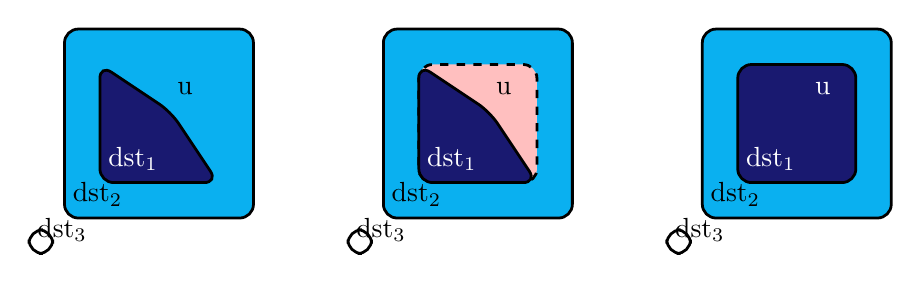
\begin{tikzpicture}[x=0.3cm, y=0.3cm,
      popped/.style={rounded corners=5pt, line width=1pt, draw, fill=MidnightBlue},
      fringe/.style={rounded corners=5pt, line width=1pt, draw, fill=ProcessBlue},
      popping/.style={rounded corners=5pt, line width=1pt, draw, dashed, fill=pink},
      unseen/.style={rounded corners=5pt, line width=1pt, draw}]
    \draw[unseen] (0,0) -- (\s,0) -- (\s,\s) -- (0,\s) -- cycle;
    \draw[fringe] (1.5,1.5) -- (9.5,1.5) -- (9.5,9.5) -- (1.5,9.5) -- cycle;
    \draw[popped] (3,3) -- (8,3) -- (6,6) -- (3,8) -- cycle;
    \node at (1.4,1) {dst$_3$};   
    \node at (2.9,2.5) {dst$_2$};   
    \node at (4.4,4) {\color{white}dst$_1$}; 
    \node at (6.6,7) {u};
    \tikzset{shift={(13.5,0)}}

    \draw[unseen] (0,0) -- (\s,0) -- (\s,\s) -- (0,\s) -- cycle;
    \draw[fringe] (1.5,1.5) -- (9.5,1.5) -- (9.5,9.5) -- (1.5,9.5) -- cycle;
    \draw[popping] (3,3) -- (8,3) -- (8,8) -- (3,8) -- cycle;
    \draw[popped] (3,3) -- (8,3) -- (6,6) -- (3,8) -- cycle;
    \node at (1.4,1) {dst$_3$};   
    \node at (2.9,2.5) {dst$_2$};   
    \node at (4.4,4) {\color{white}dst$_1$}; 
    \node at (6.6,7) {u};     

    \tikzset{shift={(13.5,0)}}

    \draw[unseen] (0,0) -- (\s,0) -- (\s,\s) -- (0,\s) -- cycle;
    \draw[fringe] (1.5,1.5) -- (9.5,1.5) -- (9.5,9.5) -- (1.5,9.5) -- cycle;
    \draw[popped] (3,3) -- (8,3) -- (8,8) -- (3,8) -- cycle;
    \node at (1.4,1) {dst$_3$};   
    \node at (2.9,2.5) {dst$_2$};   
    \node at (4.4,4) {\color{white}dst$_1$}; 
    \node at (6.6,7) {\color{white}u};       
  \end{tikzpicture}
  \caption{Popping $\m{u}$}  
\end{figure}

Next, we must account for the ripple effect that popping 
$\m{u}$ could have had on the other vertices. 
In particular, it is possible that a vertex obeying $\m{inv\_unpopped}$ can
improve its cost via $\m{u}$, and that an unreachable vertex 
obeying $\m{inv\_unseen}$ can now be reached via $\m{u}$. 
The for loop repairs these breakages by 
checking if a path via $\m{u}$ is an improvement for such vertices, and, if so, 
edits both arrays and the priority queue as seen on line~\ref{code:update}.

The for loop's invariant is similar to that of the while loop---$\m{inv\_unseen}$ 
and $\m{inv\_popped}$ are preserved as-is, modulo the popping of 
$\m{u}$ as discussed above. The key edit is in $\m{inv\_unpopped}$. blah blah blah

\colorlet{stash}{red}
\colorlet{red}{maincolor}

\begin{lstlisting}
  void dijkstra (int graph[SIZE][SIZE], int src, 
                           int *dist, int *prev) {
$//$ $\braces{\p{DijkGraph}(\gamma)}$
    int pq[SIZE];
    int i, j, u, cost;
    for (i = 0; i < SIZE; i++) {
      dist[i] = INF; 
      prev[i] = INF; 
      pq[i] = INF;
    }
    dist[src] = 0; 
    pq[src] = 0; 
    prev[src] = src;
$//$ $\braces{\p{DijkGraph}(\gamma) /| \null \\
\m{dijk\_correct}(\gamma,\m{src},\m{prev},\m{dist},\m{priq})}$
    while (!pq_emp(pq)) {
      u = popMin(pq);
      for (i = 0; i < SIZE; i++) {
        cost = graph[u][i]; 
        if (cost < INF) {
          if (dist[i] > dist[u] + cost) {
            dist[i] = dist[u] + cost;
            prev[i] = u; 
            pq[i] = dist[i];
          }
        }  
      }
    }
$//$ $\braces{\p{DijkGraph}(\gamma) /| \null \\ 
\forall \m{dst} \in \m{priq}.~\m{priq}[\m{dst}] = \texttt{INF} /| \null \\ 
\m{dijk\_correct}(\gamma,\m{src},\m{prev},\m{dist},\m{priq})}$
    return;
  }
\end{lstlisting}
\vspace{0.5em}
\begin{equation*}
\begin{split}
\p{list\_rep}(\gamma, \m{i}) &\defeq \texttt{data\_at  array  graph2mat}(\gamma)[\m{i}] \texttt{  list\_addr}(\gamma, \m{i}) \\
\vspace{1em}
\p{graph\_rep}(\gamma) &\defeq \underset{\texttt{vvalid}(\gamma,\m{v})}{\bigstar} \m{v}  \mapsto\p{list\_rep}(\gamma, \m{v})
\end{split}
\end{equation*}

\begin{equation*}
\begin{split}
\m{dijk\_correct}(\gamma, \m{src}, \m{prev}, \m{dist},& \m{priq}) \; \defeq \; \\
\forall \m{dst}.~\m{dst} \in \m{popped}(\m{priq}) \; => \; & \exists \m{path}.~\m{path\_correct}(\gamma, \m{prev}, \m{dist}, \m{path}) /| \null \\
& \m{path\_glob\_optimal}(\gamma, \m{dist}, \m{path}) /| \null \\
& \m{path\_entirely\_in\_popped}(\gamma, \m{prev}, \m{path}) /| \null \\
\m{priq}[\m{dst}] < \ifty \; => \; & \texttt{let }\m{m} \texttt{ := } \m{prev}[\m{dst}] \texttt{ in } \m{m} \in \m{popped}(\m{priq}) /| \null \\
&\forall \m{m'} \in \m{popped}(\m{priq}).~\m{cost}(\m{path2m} +:: (m, dst)) \le \null \\
&\hspace{10em} \m{cost}(\m{path2m'} +:: (m', dst)) /| \null \\
\m{priq}[\m{dst}] = \ifty \; => \; & \forall \m{m} \in \m{popped}(\m{priq}).~\m{cost}(\m{path2m} +:: (m, dst)) = \ifty
\end{split}
\end{equation*}

\colorlet{red}{stash}



	
	\section{I'm sorry Dave, I'm afraid I can't do that: Overflow}
	\label{sec:overflow}
	Dijkstra's algorithm clearly cannot work when a path
cost is more than \texttt{INT\_MAX}.  A reasonable-looking restriction
is to bound edge costs by
$\left\lfloor\frac{\texttt{INT\_MAX}}{\texttt{size}-1}\right\rfloor$, since
the longest optimal path has $\texttt{size}-1$ links and so the
most expensive possible path costs no more than \texttt{INT\_MAX}.
However, this has two flaws.  First, since we are writing real code in~C,
rather than pseudocode in an idealized setting, we must reserve some
concrete \texttt{int} value \texttt{inf} for ``infinity'', with 
the semantics that if the best-known distance to a vertex~\m{x}
is \texttt{inf}, then~\m{x} is as-yet unreachable.
A consequence of this is that reachable destination vertices cannot have a
path cost of \texttt{inf}: if they did, this would be logged in the
\texttt{dist} array and create an ambiguity.
Second, even though the best-known distances start at \texttt{inf}
(see line~\ref{code:assigninf}) and only ever decrease from there, the code can
overflow on lines~\ref{code:overflow}~and~\ref{code:update1}.

\begin{figure}[t]
\centering
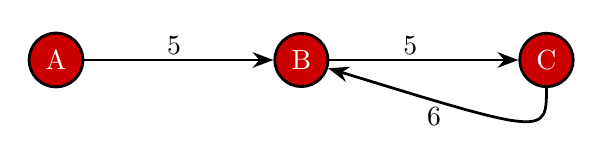
\begin{tikzpicture}[x=0.3cm, y=0.3cm,
  vert/.style={circle, line width=1pt, draw, fill=red}]
  \node[vert] (A) at (0,0) {\color{white}A};
  \node[vert] (B) [right = 8 of A] {\color{white}B};
  \node[vert] (C) [right = 8 of B] {\color{white}C};
  \draw [->,line width=1pt,arrows={-Stealth}] (A) -- (B);
  \draw [->,line width=1pt,arrows={-Stealth}] (B) -- (C);
  \draw [->,line width=1pt,arrows={-Stealth}] (C.south) .. controls ++(0, -2) .. (B);
  \node at (5,0.6) {5};
  \node at (15,0.6) {5};
  \node at (16,-2.4) {6};
\end{tikzpicture}
\caption{A graph that will result in overflow on a 4-bit machine.}
\label{fig:overflow}
\end{figure}

Consider applying Dijkstra's algorithm on a hypothetical 4-bit unsigned machine to
the graph in figure~\ref{fig:overflow}.  The \texttt{size} of the graph is 3 nodes, and so the na\"ive edge-weight upper bound is $\left\lfloor\frac{\texttt{INT\_MAX}}{\texttt{size}-1}\right\rfloor = \left\lfloor\frac{15}{3-1}\right\rfloor = 7$, for example as in the graph pictured in figure~\ref{fig:overflow}.  Indeed, a glance at the figure is enough to tell that the true distance from the source~A~to vertices~B~and~C~are~5~and~10 respectively---both of which are representable with 4 bits, and so na\"ively all seems well.  %Unfortunately, Dijkstra's algorithm does not exactly work like that.
Indeed, after processing vertices~A~and~B, 5~and~10~\emph{are} the costs reflected in the \texttt{dist} array for~B~and~C respectively---\emph{but unfortunately vertex~C~is still in the priority queue}.  After vertex~C~is popped on line~\ref{code:pop}, we fetch its neighbors in the \texttt{for} loop; the cost from C~to~B~(6)~is fetched on line~\ref{code:cost}.  On line~\ref{code:overflow} the currently optimal cost to~B~(5) is compared with the sum of the optimal cost to~C~(10) plus the just-retrieved cost of the edge from~C~to~B~(6).  Since $10+6$ overflows in 4-bit arithmetic, the comparison is not between~5~and~16 but in fact between~5~and~0!  Thus the code decides that a new cheaper path from~A~to~B~exists (in particular, A$\leadsto$B$\leadsto$C$\leadsto$B) and then trashes the \texttt{dist} and \texttt{prev} arrays on line~\ref{code:update1}.

Our code uses signed \texttt{int} rather than \texttt{unsigned int} so we have undefined behavior rather than defined-but-wrong behavior, but the essence of the overflow is identical.
Our solution is twofold.  First, we restrict the maximum edge cost to $\left\lfloor\frac{\texttt{INT\_MAX}}{\texttt{size}}\right\rfloor - 1$, which in the 4-bit setting just described forces an edge cost of no more than~4.  Consider modifying figure~\ref{fig:overflow} to
have edge weights of~4~rather than~5s~and~6s.  After processing vertices~A~and~B, the distances to~B~and~C are no more than~4~and~8 respectively.  When we process vertex~C, the comparison on line~\ref{code:overflow} is thus between the previous best cost to~B~(4) and the candidate best cost to~B~via~C~(12); there is no overflow and the code behaves as advertised.

The second part of our solution is that we require in the function precondition that $\left\lfloor \frac{\texttt{INT\_MAX}}{\texttt{size}} \right\rfloor - 1 < \texttt{inf} \le \texttt{INT\_MAX} - \left\lfloor \frac{\texttt{INT\_MAX}}{\texttt{size}} \right\rfloor + 1$.  As long as $\texttt{size} > 1$, this is perfectly realizable  by setting \texttt{inf} to $\texttt{INT\_MAX} - \left\lfloor \frac{\texttt{INT\_MAX}}{\texttt{size}} \right\rfloor + 1$, \emph{i.e.} in the 4-bit machine we set \texttt{inf} to $11$.  When $\texttt{size} = 1$, this inequality is not realizable; our verification is thus not applicable to single-vertex graphs, a special case for which the shortest-path problem is in any event rather uninteresting.


	
	\section{Extension of CertiGraph for undirected graphs}
	\label{sec:undirected}
	\subsection{Graph definition in CertiGraph}

\begin{lstlisting}
Record PreGraph {EV: EqDec Vertex eq} {EE: EqDec Edge eq} := {
	vvalid : Ensemble Vertex;
	evalid : Ensemble Edge;
	src : Edge -> Vertex;
	dst : Edge -> Vertex
}.
\end{lstlisting}
In CertiGraph, every graph has the four following basic functions: $vvalid$ which determines which vertices are valid in the graph; $evalid$ which determines which edges are valid in the graph, and two functions $src$ and $dst$ to map each edge to vertices. For example, an edge $e$ in graph $g$ pointing from vertex $u$ to $v$ will have $src$ $g$ $e$ $=$ $u$ and $dst$ $g$ $e$ $=$ $v$. What these functions actually are, is defined during the actual construction of a graph.

As a result of this definition, the graphs defined in our library are effectively directed - each valid edge in the graph has a clear direction defined by the $src$ and $dst$ functions. This makes sense in most use cases, especially when reasoning about C pointers.

The issue is how then to reason about undirected graphs in a library whose graphs are directed by design. Undirected graphs are generally treated as a separate kind of graph from directed graphs. Thus, the most naive idea is to consider undirected edges as a separate category from directed edges, by introducing a new \texttt{Ensemble} for undirected edges. This has the benefit of reasoning with multigraphs that contains both directed and undirected edges. However, as most of our graphs are either directed or undirected, it will be unwieldy for a graph to have to maintain ensembles of both kinds of edges when it will never use one kind. Furthermore, it requires us to recreate many fundamental operations for manipulating edges, ignoring the already robust suite of lemmas we have for $evalid$, $src$ and $dst$.

Instead, we decided to rely on the observation that \textit{every directed graph can be treated as an undirected graph} by simply ignoring the directions of the edges. That is, we can assert that a graph in our library, directed by default, holds certain undirected graph properties. This is backed by our observation that undirected graph properties are largely mathematical in nature and, depending on the representation, have few to no spatial requirements in separation logic. Furthermore, there is no overlap in their properties - claiming that directed graph holds an undirected graph property by ignoring the direction of its edges, does not affect its directed properties. It also allows us to use our rich set of directed-graph lemmas about the addition and removal of edges.

\subsection{Undirected graph properties}

Here we give a quick explanation of the main undirected definitions and properties we're interested in. Our definitions are largely based on CLRS~\cite{clrs}.

Let $g$ be a graph. A valid edge $e$ in $g$ is an adjacent edge (or \textit{adj\_edge} for short) of valid vertices $u$ and $v$ if those are its $src$ and $dst$. $u$ and $v$ are \textit{adjacent} if such an edge exists in $g$.
\begin{lstlisting}
Definition adj_edge (g: PreGraph V E) (e: E) (u v: V) :=
	strong_evalid g e /\
	((src g e = u /\ dst g e = v) \/ (src g e = v /\ dst g e = u)).

Definition adjacent (g: PreGraph V E) (u v: V) :=
	exists e: E, adj_edge g e u v.
\end{lstlisting}
A similar approach is proposed in Halsbeck~\cite{DBLP:journals/afp/HaslbeckLB19}.

A valid undirected path, or \textit{upath}, in $g$ is a list of vertices such that each vertex in the list is adjacent with the subsequent vertex. An empty path, $nil$, is by default a valid $upath$. A singleton path $[v]$ is also a valid $upath$ if $v$ is a valid vertex.
\begin{lstlisting}
Fixpoint valid_upath (g: PreGraph V E) (p: upath) : Prop :=
match p with
| nil => True
| u :: nil => vvalid g u
| u :: ((v :: _) as p') => adjacent g u v /\ valid_upath g p'
end.
\end{lstlisting}
Two vertices $u$ and $v$ are \textit{connected by p} if $p$ is a valid $upath$ in $g$ with the head vertex $u$ and last vertex $v$. They are \textit{connected} if such a $upath$ exists. By the above, every valid vertex in $g$ is trivially connected to itself.
\begin{lstlisting}
Definition connected_by_path (g: PreGraph V E) (p: upath) (n : V) :=
	fun n' => valid_upath g p /\
		hd_error p = Some n /\ last_error p = Some n'.

Definition connected (g: PreGraph V E) (n : V) :=
	fun n' => exists p, connected_by_path g p n n'.
\end{lstlisting}
An undirected cycle, or $ucycle$, is a $upath$ whose first and last vertices are the same. A $simple$ $upath$ is a valid $upath$ that has no duplicate vertices - no vertex is visited twice. A $simple$ $ucycle$ is a cycle whose tail has no duplicate vertices - the only "duplicates" in the cycle are the first and last vertices.

Note that the definition of path varies between textbooks and papers. For example, \textit{Discrete Mathematics and its Applications}~\cite{rozen} define paths as a sequence of edges with an implicit sequence of vertices, whereas CLRS, which we have followed, defines it as a sequence of vertices with an implicit sequence of edges.

\subsection{Defining forests before trees}

CLRS defines a tree as "a (connected) graph with no simple undirected cycles" - in other words, a connected, acyclic graph. We use the same definition:
\begin{lstlisting}
Definition uforest g:=
	(forall e, evalid g e -> strong_evalid g e) /\
	(forall p l, $\neg$ simple_ucycle g p l).
\end{lstlisting}
Our definition contains two propositions. The first constrains a forest to have no excess, "dangling" edges. Although our graph library needs to reason about such edges, we do not want to tolerate them in our forests. The second is the key "no simple undirected cycles".
\begin{figure}[H]
	\begin{tikzpicture} [auto, node distance =1.5 cm and 1.5cm ,on grid, semithick, state/.style ={ circle}]
		\node[state] (V0) {$V0$};
		\node[state] (V1) [right=of V0] {$V1$};
		\node[state] (V2) [below=of V0] {$V2$};
		\node[state] (?1) [above=of V0] {$?$};
		\node[state] (?2) [right=of V1] {$?$};
		\node[state] (?3) [below right=of ?2] {$?$};
		\path (V0) edge node[above=0.15 cm] {$5$} (V1);
		\path (V0) edge node[left=0.15 cm] {$6$} (V2);
		\path (V0) edge node[left=0.15 cm] {$-1$} (?1);
		\path (?2) edge node[above right=0.15 cm] {$2$} (?3);
	\end{tikzpicture}
	\caption{The above is not a forest, due to the "dangling" edges (? being a placeholder for invalid vertices)}
\end{figure}
We also highlight a difference in our definition compared to mathematical textbooks. Prim's and Kruskal's algorithms are presented as minimum-spanning \textit{tree} algorithms, and often have the implicit assumption that the graph is fully connected. They may or may not discuss forests - CLRS does not, while \textit{Discrete Mathematics} informally defines forests as ``containing no simple circuits that are not necessarily connected [...] and have the property that each of their connected components is a tree." In short, these sources define forests from ``bottom-up" using trees. Our ``top-down" definition instead recognises forests as acyclic graphs, and trees as a special case of forests where every vertex is connected to each other. This definition was also used by Lammich et al~\cite{DBLP:journals/afp/LammichN19}.
\begin{lstlisting}
Definition connected_graph (g: PGraph) :=
	forall u v, vvalid g u -> vvalid g v -> connected g u v.

Definition utree g := uforest g /\ connected_graph g.
\end{lstlisting}
	
	\section{Verified Prim in C}
	\label{sec:prim}
	Here we discuss our verifications of the classic MST algorithms Prim and Kruskal.  Although our machine-checked proofs are about real~C~code, in this section we take a higher-level approach than we did in \S\ref{sec:dijkstra}, focusing on our key algorithmic findings and overall experience.  Accordingly, we only provide pseudocode for Prim's algorithm rather than a decorated program and do not show any code for Kruskal's.  Our development contains our~C~code and formal proofs~\cite{anonrepo}.

%\vspace*{-0.25em}

\subsection{Prim's Algorithm}
\label{sec:prim}

%\vspace*{-0.25em}

\begin{figure}[t]
\[
\begin{array}{@{}l@{~~}|@{~~}l@{}}
\begin{minipage}{0.475\textwidth}
\begin{lstlisting}
MST-PRIM(G,w,r):
 for each u in G.V
  u.key = INF
  u.parent = NIL $\hide{code:primsetinitparent}$
 r.key = 0 $\label{code:primsetroot}$
 Q = G.V
 while Q $\neq$ $\emptyset$
  u = EXTRACT-MIN(Q) $\hide{code:primextractmin}$
  for each v in G.Adj[u]
   if v $\in$ Q and w(u,v) $<$ v.key
    v.parent = u
    v.key = w(u,v) $\hide{code:primeditpri}$
\end{lstlisting} \end{minipage} &
\begin{minipage}{0.5\textwidth}
\begin{lstlisting}[numbers=none]
MST-NOROOT-PRIM(G,w):
 for each u in G.V
  u.key = INF
  u.parent = NIL

 Q = G.V
 while Q $\neq$ $\emptyset$
  u = EXTRACT-MIN(Q)
  for each v in G.Adj[u]
   if v $\in$ Q and w(u,v) $<$ v.key
    v.parent = u
    v.key = w(u,v)
\end{lstlisting}
\end{minipage}
\end{array}
\]
%\vspace*{-1.25em}
\caption{Left: Prim's algorithm from CLRS~\cite{clrs}. Right: the same omitting line 5.}
%\vspace*{-1.25em}
\label{fig:prims}
\end{figure}

We put the pseudocode for Prim's algorithm in figure~\ref{fig:prims}; the code on the left-hand side is directly from CLRS, whereas the code on the right omits line 5 and will be discussed in~\S\ref{sec:primforest}.  Note that line 12 contains an implicit call to the PQ's \texttt{edit\_priority}.  Since the pseudocode only compares \texttt{key}s (\emph{i.e.}, edge weights) rather than doing arithmetic on them \emph{\`a la} Dijkstra, there are no potential overflows and it is reasonable to set \texttt{INF} to \texttt{INT\_MAX} in~C.

Indeed, our initial verifications of~C~code were largely ``turning the crank'' once we had the definitions and associated lemma support for pure/abstract undirected graphs, forests, \emph{etc.} discussed in \S\ref{sec:newundirected}.  Accordingly, our initial contribution was a demonstration that this new graph machinery was sufficient to verify real code.  We also proved that our extensions to CertiGraph from~\S\ref{sec:extensions} were generic rather than verification-specific by reusing much pure and spatial reasoning that had been originally developed for our verification of Dijkstra.

%\vspace*{-0.25em}

\subsection{Prim's Algorithm handles multiple components out of the box}
\label{sec:primforest}

%\vspace*{-0.25em}

Textbook discussions of Prim's algorithm are usually limited to single-component input graphs (\emph{a.k.a.} connected graphs), producing a minimum spanning tree.  It is widely believed that Prim's is not directly applicable to graphs with multiple components, which should produce a minimum spanning forest.  For example, both Rozen~\cite{rozen} and Sedgewick \emph{et al.}~\cite{sedgewick,DBLP:books/daglib/0029345} leave the extension to multiple components as an formal exercise for the reader, whereas Kepner and Gilbert suggest that multiple-component graphs should be handled by first finding the components and then running Prim on each component~\cite{kepnergilbert}.  This appears to be the standard solution, appearing in numerous lectures and implementations\footnote{Another standard solution is to use Kruskal's \hide{or Boruvka's~\cite{boruuvka1926jistem}} algorithm instead.}. %CLRS does not mention the case of disconnected graphs

After we completed our initial verification, a close examination of our formal invariants showed us that the algorithm \emph{exactly as given by standard textbooks} will properly handle multi-component graphs \textit{in a single run}.  The confusion starts because, in a fully connected graph, any vertex $\texttt{u}$ removed from the PQ on line~8 must have $\texttt{u.key} < \texttt{INF}$; \emph{i.e.}, $\texttt{u}$ must be immediately reachable from the spanning tree that is in the process of being built.  However, nothing in the code relies upon this connectedness fact!  All we need is that $\texttt{u}$ is the ``closest vertex'' to the ``current component.''  If $\texttt{u.key}=\texttt{INF}$ \emph{and} \texttt{u} is a minimum of the PQ, then it simply means that the ``previous component'' is done, and we have started spanning tree construction on a new unconnected component ``rooted'' at \texttt{u}, yielding a forest.  The node $\texttt{u}$'s parent will remain \texttt{NIL}, at it was after the setup loop on line~4, indicating that it is the root of a spanning tree.  Its \texttt{key} will be $\texttt{INF}$ rather than $0$, but the \texttt{key}s are \emph{internal to Prim's algorithm}: clients only get back the spanning forest as encoded in the \texttt{parent} pointers\footnote{The \texttt{key}s simply record the edge-weight connecting a vertex to its candidate parent; recall that line~12 is really a call to the PQ's \texttt{edit\_priority}.  If a client wishes to know this edge weight, it can simply look up the edge in the graph.}.

Having made this discovery, we updated our proofs to support the new weaker precondition, which is what we currently formally verify in Coq~\cite{Coq}.
A little further thought led to the realization that since Prim can handle arbitrary numbers of components, the initialization of the root's \texttt{key} in line~5 is in fact unnecessary.  Accordingly, if we remove this line and the associated function argument \texttt{r} from \texttt{MST-PRIM} (\emph{i.e.}, the code on the right half of figure~\ref{fig:prims}), the algorithm still works correctly.  Moreover, \emph{the program invariants become simpler} because we no longer need to treat a specified vertex (\texttt{r}) in a distinguished manner.  Our formal development verifies this version of the algorithm as well~\cite{anonrepo}.

\subsection{Related work on Prim in algorithms and formal methods}
\label{sec:relworkprim}

Prim's algorithm was in fact first developed by the Czech mathematician Vojt\v{e}ch Jarn\'{i}k in 1930~\cite{prim1:jarnik} before being rediscovered by Robert Prim in 1957~\cite{prim2:prim} and a third time by Edsger~W.~Dijkstra in 1959~\cite{prim3:dijkstra}.  Both Prim's and Dijkstra's treatment explicitly assumes a connected graph; although we cannot read Czech, some time with Google translate suggests that Jarn\'{i}k's treatment probably does the same.  The textbooks we surveyed \cite{kepnergilbert,sedgewick,DBLP:books/daglib/0029345,rozen,DBLP:books/daglib/0022194,clrs,DBLP:books/daglib/0015106} seem to derive from Prim's and/or Dijkstra's treatment.
More casual references such as Wikipedia~\cite{prim:wiki} and innumerable lecture slides are presumably derived from the textbooks cited.  We have not found any references that state that Prim's algorithm \emph{without modification} applies to multi-component graphs, even when executable code is provided: \emph{e.g.}, Heineman \emph{et al.} provide C++ code that aligns closely with our C code~\cite{heineman2008algorithms}, but do not mention that their code works equally well on multi-component graphs.  Indeed, many sources promulgate the false proposition that modifications to the algorithm are needed to handle multi-component graphs (\emph{e.g.},~\cite{kepnergilbert,sedgewick,DBLP:books/daglib/0029345,rozen,prim:wiki}).  Likewise, we have found no reference that removes the initialization step (line~5~in figure~\ref{fig:prims}) from the standard algorithm.

Prim's algorithm has been the focus of a few previous formalization efforts.  Guttman formalised and proved the correctness of Prim's algorithm using Stone-Kleene relation algebras in Isabelle/HOL~\cite{DBLP:conf/ictac/Guttmann16}.  He works in an idealized formal environment that does not require the development of explicit data structures; his code does not appear to be executable.  Lammich \emph{et al.} provided a verification of Prim's algorithm~\cite{DBLP:journals/afp/LammichN19}.  Lammich \emph{et al.} also work within the idealized formal environment of Isabelle/HOL, but in contrast to Guttman develop efficient purely functional data structures and extract them to executable code.  Both Guttman and Lammich explicitly require that the input graph be connected. % and produce a tree.

%axiomatizes
%his second paper that their earlier proof of Prim's assumed "".



%  We make two immediate observations on CLRS's pseudocode: first, that they do not give an explicit definition for

% Note that  does not explicitly define \texttt{EXTRACT-MIN}

%are often limited to the case where the input graph is a connected graph. This is reasonable, as their purpose is to teach the concept of minimum-spanning \textit{tree} algorithms. However, they seldom expand on the subject of spanning forests for disconnected graphs. For example, . \textit{Discrete Mathematics and Its Applications} leaves it as an exercise to the reader, while \textit{Graph Algorithms in the Language of Linear Algebra}~\cite{kepnergilbert} suggests running Prim's on each component of the disconnected graph to obtain a minimum spanning forest. The last appears to be the most common solution, with suggesting this.


\hide{
\begin{figure}[H]
\begin{tikzpicture} [auto, node distance =2 cm and 2cm ,on grid, semithick, state/.style ={circle}]
\node[state] (V0) {$\m{v_0}$};
\node[state] (V1) [right=of V0] {$\m{v_1}$};
\node[state] (V2) [below=of V0] {$\m{v_2}$};
\node[state] (V3) [below right=of V0] {$\m{v_3}$};
\node[color=green] (V4) [right=of V3] {$\m{v_3}$};
\node[color=green] (V5) [right=of V4] {$\m{v_5}$};
\draw[color=red] (V0) edge [ultra thick] node[above=0.15 cm] {$5$} (V1);
\path (V0) edge node[left=0.15 cm] {$6$} (V2);
\path (V0) edge [thin] node[above right=0.05 cm] {$5$} (V3);
\path[color=red] (V1) edge [ultra thick] node[right=0.15 cm] {$5$} (V3);
\path[color=red] (V2) edge [ultra thick] node[below=0.15 cm] {$4$} (V3);
\path (V4) edge node[below=0.15 cm] {$1$} (V5);
\end{tikzpicture}
\caption{Figure of a partial Prim's execution with root $\m{v_0}$. A spanning tree for the left component has been found as indicated in red, while $\m{v_4}$ and $\m{v_5}$ are in the priority queue with weight \texttt{INF}. As our \texttt{EXTRACT-MIN} tolerates \texttt{INF}, our implementation will pop them from the priority queue and proceed as usual, instead of terminating with only the left tree.}
\end{figure}

From the above figure, we demonstrate that our simple priority queue will always pop vertices regardless of its weight. If the popped vertex has weight \texttt{INF}, its parent will also be at its default invalid value, indicating that no edge was added to the graph. We then continue the algorithm as usual, updating the weights of adjacent vertices. As a result, our Prim implementation can return a minimal spanning forest without ``premature termination".

Is our assumption that \texttt{EXTRACT-MIN} can pop \texttt{INF} weight vertices reasonable? We argue that it is, because the abstract algorithm in CLRS makes no statement about \texttt{INF} beyond the initialization. As the algorithm pushes the vertices into queue with weight \texttt{INF}, it is reasonable to say the priority queue can tolerate items with weight \texttt{INF}. Doing so simplifies \texttt{EXTRACT-MIN} to a \texttt{popMin} operation using the priority queue's API, without requiring additional lines of code to further check for specific weights.

Consequently, our code allows a simple implementation of Prim's to return a forest for a disconnected input graph, in a single run of the algorithm without needing to identify the disconnected components beforehand. It is important to note that we do not explicitly define ``components", nor do we tag \texttt{u} as a``new root". It is sufficient to prove that the loop invariant is satisfied whether \texttt{key[u]~< INF} or \texttt{key[u] = INF}.

Note that the priority queue used for this verification is still tied to \texttt{INF}, and thus in the verification our argument is weakened to ``\texttt{INF} is a valid weight in the priority queue" rather than ``membership in the priority queue is independent of \texttt{INF}". Work on a stronger priority queue which completely dissociates from \texttt{INF} was to be delivered by Aquinas Hobor since May 2020.
}

%  If they wish to determine the edge cost from a node to its parent, they can look it up in the graph, with the special case

%We observed that our code is able to return a minimum spanning forest when the input graph is disconnected, . The reason for this is: We treat a vertex of weight \texttt{INF} and a vertex's membership in the priority queue as \textit{separate} matters. A vertex can be in the priority queue with weight \texttt{INF}, represented by \texttt{key[u] = INF}, and this indicates that \texttt{u} is \textit{not} connected to any previously popped vertex; otherwise its weight would have been previously lowered. However, our priority queue does not care about its items having specific weights, only that the item it pops is always the one with the lowest weight. Thus, when a vertex \texttt{u} is returned, it is possible that \texttt{u} has weight \texttt{INF} - the scenario where all vertices remaining in the queue has weight \texttt{INF}, indicating all of them are disconnected from the current forest.

%Rather than start with a distinguished root vertex, we simply start with zero components, and the first vertex we extract (chosen arbitrarily by the PQ) becomes the root of the initial

%A further observation is that if we dissociate \texttt{INF} and the priority queue, then the input root required by Prim's is no longer necessary. The root's key is artificially set to 0 in Prim's, which kickstarts the main loop. However, since our emptiness check and \texttt{EXTRACT-MIN} implementation can return vertices with \texttt{INF} weight, the loop will start as long as there are un-popped vertices. Thus, we suggest it is possible to remove the \texttt{rt} parameter. Doing so simplifies the proof, because we do not have to reason about the artificially weighted \texttt{key[rt]}. The noroot-variant is in Figure 4 at the beginning of this section, while the verified implementation of Prim's without root is in \texttt{noroot\_prim.c}.

%They push their version of \texttt{INF} into the priority queue during the setup, and do not perform any explicit rejections of \texttt{INF}, simply popping from the priority queue at the \texttt{EXTRACT-MIN} step. However, they do not discuss minimum spanning forests, hence this observation is not recorded.

	
	\section{Verified Kruskal in C}
	\label{sec:kruskal}
	\subsection{Kruskal's Algorithm}
\label{sec:kruskal}

Although Kruskal's algorithm is sometimes presented as taking connected graphs and producing spanning trees, the literature also discusses the more general case of multi-component input graphs and spanning forests.  However, Kruskal has only recently been the focus of formal verification efforts, partly because it relies on the notoriously difficult-to-verify union-find algorithm; fortunately, the CertiGraph project has an existing fully-verified union-find implementation that we can leverage~\cite{DBLP:journals/pacmpl/WangCMH19}.  Kruskal also requires a sorting function; we implemented \texttt{heapsort} as explained in \S\ref{sec:heapsort}.  Kruskal is optimized for compact representations of sparse graphs, so the $O(1)$ space cost of \texttt{heapsort} is a reasonable fit.  %Including the code for union-find and heap sort, the code for Kruskal's algorithm is around 200 lines of~C.

The primary interest of our verification of Kruskal is in our proof engineering.  Kruskal inputs graphs as edge lists rather than adjacency matrices.  In addition to requiring an addition to our spatial graph predicate menu, this means that Kruskal's input graphs can have multiple edges between a given pair of vertices (\emph{i.e.}, a ``multigraph'').  Pleasingly, we can reuse most of the undirected graph definitions (\S\ref{sec:newundirected}), demonstrating that they are generic and reusable.

Another challenge is integrating the pre-existing CertiGraph verification of union-find.  We are pleased to say that no change was required for CertiGraph's existing union-find definitions, lemmas, specifications and verification.  Kruskal actually manipulates two graphs simultaneously: a directed graph with vertex labels (to store parent pointers and ranks) within union-find, and an undirected multigraph with edge labels (for which the algorithm is constructing a spanning forest).  Beyond showing that CertiGraph was capable of this kind of systems-integration challenge, we had to develop additional lemma support to bridge the directed notion of ``reachability,'' used within the directed union-find graph to the undirected notion of ``connectedness,'' used in the MSF graph (\S\ref{sec:newundirected}).

%notions of  as defined and ; with  as defined and }.

%\subsection{Reusing previously verified union-find} %%why is there such an absurdly large space?
%Kruskal's algorithm requires a union-find data structure to keep track of the state of connectedness in the partial forest. Since CertiGraph had published several verified union-find implementations, we decide to make use of them. However, as these implementations had no client using them until now, we discovered that the postconditions of the union-find calls were difficult to use for Kruskal's verification. The union-find implementations were verified prior to our introduction of undirected graph properties, thus were not designed with connectedness in mind.

%To that end, we have extended lemmas about the results of union-find operations as an analog to connectivity. We are pleased to say that no change was required for Wang's existing union-find definitions, lemmas, specifications and verification. Instead, we proved that their existing postconditions mathematically imply an analog to connectivity in undirected graphs. In other words, Wang's verified postconditions were \textit{not} incorrect or poor, they just required mathematical translation into what we wanted in the context of Kruskal's.

%We mention this to emphasise the modularity and buildability of VST and CertiGraph infrastructure - that we were able to use previously, independently proven code in a bigger system later. The internal details and verification of the union-find system are independent from that of Kruskal's, whose proof only required the preconditions and postconditions of whichever union-find implementation we decide to use.

\subsection{Related work on Kruskal in algorithms and formal methods}
\label{sec:relworkkruskal}

Joseph Kruskal published his algorithm in 1956~\cite{kruskal} and it has appeared in numerous textbooks since (\emph{e.g.},~\cite{clrs,DBLP:books/daglib/0022194,sedgewick,DBLP:books/daglib/0015106}).  Kruskal's algorithm is usually preferred over Prim's for sparse graphs, and is sometimes presented as ``the right choice'' when confronted with multi-component graphs under the mistaken assumption that Prim's first requires a component-finding initial step.

Guttman generalised minimum spanning tree algorithms using Stone relation algebras~\cite{DBLP:journals/jlp/Guttmann18}, and provided a proof of Kruskal's algorithm formatted in said algebras.  Like his work on Prim's~\cite{DBLP:conf/ictac/Guttmann16}, Guttmann works within Isabelle/HOL and does not include concrete data structures such as priority-queues and union-find, instead capturing their action as equivalence relations in the underlying algebras. In Guttmann's Kruskal paper, he mentions that his Prim paper axiomatizes the fact that ``every~finite~graph has~a~minimum~spanning~forest,'' which he is then able to prove \emph{using his Kruskal algorithm}.  Interestingly, our Prim verification needs the same fact, but we prove it directly. % that every finite graph has a finite, nonempty list of spanning forests.

In a similar vein, Haslbeck \emph{et al.} verified Kruskal's algorithm~\cite{DBLP:journals/afp/HaslbeckLB19} by building on Lammich \emph{et al.}'s earlier work on Prim~\cite{DBLP:journals/afp/LammichN19}.  Like Lammich \emph{et al.}, Haslbeck \emph{et al.} work within Isabelle/HOL with a focus on purely functional data structures.

One of the stumbling blocks in verifying Kruskal's algorithm is the need to verify union-find.  In addition to CertiGraph, 

%In Lammich et al, their Prim's implementation explicitly expects a connected graph, and they do not reason about the disconnected case.

%Working in an idealized formal environment, they do not require the development of .

%\note{Despite this connectedness requirement, Guttman stated in a subsequent paper~\cite{DBLP:journals/jlp/Guttmann18} that his proof of Prim in~\cite{DBLP:conf/ictac/Guttmann16} asserts that  as an axiom.}

%Guttman later proved this by relying on their proof of Kruskal's. We use the same assertion in our proof of Prim's, but in our case, Kruskal's is defined in the spatial layer of our library, not the mathematical-layer, and it would be unwieldy to bring it back up. Instead, we show in the mathematical layer that  Thus there exists a minimum spanning forest by simply taking the minimal-weight forest in this list. 

	\section{Structure of graph library}
	\label{sec:structure}
	Verifying real code is meaningfully harder than verifying toy implementations.  On top of such challenges, verifying graph algorithms requires a significant amount of mathematical machinery: there are many plausible ways to define basic notions such as reachability, but not all of them can handle the challenges of verifying real code~\cite{shengyi:thesis}.  Moreover, we would like our mathematical, spatial, and verification machinery to be generic and reusable.

All of the above suggests that it is important to work within existing formal proof developments due a strong desire to not reinvent very large wheels (the existing proof bases we work with contain hundreds of thousands of lines of formal proof).  We chose to work with the CompCert certified compiler~\cite{leroy:compcert}; the Verified Software Toolchain~\cite{appel:programlogics}, which provides significant tactic support for separation logic-based deductive verification of CompCert~C programs; and the CertiGraph framework~\cite{DBLP:journals/pacmpl/WangCMH19}, which provides much pure and spatial reasoning support for verifying graph-manipulating programs within VST.  We did so because these frameworks can handle the challenges of real code and because the CertiGraph included several fully verified implementations of union-find that we wished to reuse in our verification of Kruskal's algorithm.

Modular formal proof development involves major software engineering challenges~\cite{DBLP:journals/corr/abs-2003-06458}.
Accordingly, we took care factoring our extensions to CertiGraph into generic and reusable pieces.  This factoring allows us to reuse machinery between verifications, including in the mathematical, spatial, and verification levels, so \emph{e.g.} we share significant pure and spatial machinery between Dijkstra, Prim, and Kruskal.  Moreover, we maintain good separation between pure and spatial reasoning, so \emph{e.g.} both our Dijkstra and Prim verifications can handle multiple spatial variants of adjacency matrices without significant change.

On the other hand, working within existing developments involves some challenges, primarily in that some design decisions have been already made and are hard to change.  Moreover, our verifications tickled numerous bugs within VST, including: overly-aggressive automatic entailment simplifying, poor error messages, improper handling of~C~\texttt{struct}s, and performance issues.  We have been fortunate that the VST team has been willing to work with us to fix such bugs, although some work still remains.  Performance remains one area of focus: for example, checking our verification of Kruskal with a 3.7GHz processor and 32gb of memory takes more than 22 minutes even after all of the generic pure and spatial reasoning has been checked, \emph{i.e.} approximately 7 seconds per line of~C~code (including whitespace and comments).  This performance is unviable for verifying an industrial-sized application of equivalent difficulty: \emph{e.g.}, it would take 13 years for Coq to check the proof for 1,000,000 lines of~C.  Before some optimizations to our proof structure, the time was significantly longer still.

%\subsection{Working within large existing frameworks}




%\subsection{Structure of graph library}
\label{sec:structure}

%\subsection{Modularity of library and VST verification}
%In previous work by both VST and CertiGraph, the C functions and algorithms implemented and verified are isolated programs with little to no dependency on each other. Even the garbage collector verified by Wang et al was independent of the other verified algorithms in the library. VST has noted the importance of having a client for a verified program, to judge whether the actual utility of the verified specifications\cite{DBLP:conf/iwmm/AppelN20}. Our work on Kruskal's algorithm is the first step in verifying code that uses \textit{previously} verified C code. To make use of Wang's verified union-find, we reorganised the internal hierarchies in his CertiGraph library, providing a clearer separation between mathematical lemmas, VST specifications and proofs.

%\includegraphics[scale=0.50]{structure_placeholder.jpg} %Please check in this file.

%We reorganised CertiGraph into three layers: The mathematical layer which contains ``pure Coq" mathematical models and lemmas; the spatial layer to represent graphs in Verifiable C; and the verification layer, for specifications and verifications of C code, whose ASTs were retrieved from CompCert's \textit{clightgen} utility. We further separate this third layer into specifications and verifications. This allows reuse of a previous specification by another system without being burdened by the verification, as illustrated above. The development and verification of components can then be performed in parallel.

%In addition, we have worked to improve on the modularity of the mathematical layer, ensuring that similar graph properties and lemmas can be reused by different proofs with little need for repetition.

\subsection{Size of our development}
Our new contributions to CertiGraph include approximately:
\begin{itemize}
\item2000 lines of lemmas of undirected graph properties
\item200 lines to link unionfind properties with undirected graph properties
\item1500 lines for mathematical properties of graphs that fit in symmetric matrices, including a proof of the existence of minimal spanning forests
\item900 lines for that of edge lists
\item1800 lines \textit{each} for the verification of Prim's and Kruskal's algorithms, including the mathematical proofs of the resultant forest's minimality and helper C functions.
\end{itemize} 

	\section{Observations of VST}
	\label{sec:vst}
	\subsection{Speed of loop invariants}
The recommended tactic to solve invariants and ENTAIL goals in VST is \textit{entailer!}. However, we observed that our invariants contained a significiant number of mathematical statements, encoded by VST as PROPs, that were difficult to solve with VST's \textit{entailer!} tactic. As a result, \textit{entailer!} often took a long time to solve or reduce the invariant. To overcome this, we had to pre-solve every PROP in the invariant and preformat the SEP clauses. In the most significant case, an \textit{entailer!} call that took 446 seconds and still returned a large number of unsolved PROPs, was reduced to 36 seconds at the fastest recorded. (Tested on a VirtualBox Lubuntu 18.04 machine assigned 8GB RAM and 2 processors)

That the tactic could not solve many of our invariant \texttt{PROP}s by itself was expected and reasonable, as they were often complex properties of graphs. However, we were surprised that several solved \texttt{PROP}s took a significant amount of time despite being trivial at first glance. This is especially noticed in PROPs with preconditions of elements in empty lists. Thus, an immediate suggestion to the \textit{entailer!} tactic is to test "\textit{try contradiction}" as early as possible.
\begin{lstlisting}
assert (Hinv_10: forall u v : V,
	In u (nil (A:=V)) -> In v (nil (A:=V)) ->
	connected g u v <-> connected edgeless_graph' u v). {
		intros. contradiction.
}
\end{lstlisting}
The above Coq assertion in our loop precondition, which was easily solved by two basic tactics, cost an additional 50s when left to \textit{entailer!} to prove.
\newline\newline
Given the possibility that invariants carry PROPs on abstract graph properties that we do not expect \textit{entailer!} to solve, a thought is to provide a reduced version of \textit{entailer!} that does not reason about PROPs at all, but leaves them to the user to solve, and focuses on more VST-specific issues such as SEP and LOCAL clauses. This will be useful for verification of functions that implement abstract models.

\subsection{Shared clightgen issue with libraries.} It is obvious that one must include the dependencies of the program when compiling C code. However, we observe an issue of the opposite nature in VST and CompCert - that when running \textit{clightgen} for a program, one must include all programs using the same dependency to properly regenerate the AST file of said dependency. Failure to do so results in the proof of the other program failing to run.

For instance, in the above figure, both Dijkstra's and Prim's implementations are dependent on the same verified priority queue. When running clightgen for Prim's, we include the priority queue's C implementation to regenerate the AST tree. However, without including Dijkstra's in the same command, the existing verification of Dijkstra's experiences an error over the priority queue's newly regenerated AST file.

This is a hindrance to the modular design we aspire to, and we believe is worth looking into, to see if the error is caused by a trivial matter in CompCert's clightgen or worse.
	
	%% If you have bibdatabase file and want bibtex to generate the
	%% bibitems, please use
	%%
	%\bibliographystyle{plainurl}% the mandatory bibstyle
	
	\section{Concluding thoughts: Future and Related Work}
	\label{sec:conclusion}
	\subsection{Related work}

We have already discussed work directly related Dijkstra's (\S\ref{sec:relworkdijkstra}), Prim's (\S\ref{sec:relworkprim}), and Kruskal's (\S\ref{sec:relworkkruskal}) algorithms in detail, including work from both the algorithms and formal methods literature.  Briefly to the point of unreasonableness, our observations about Dijkstra's overflow and Prim's specification are novel, and existing formal proofs focus on code working within idealized environments rather than handling the real-world considerations that we do.  We have also already discussed the three formal developments we
build upon and extend: CompCert, VST, and CertiGraph (\S\ref{sec:stats}).  Our goal now is to discuss mechanized graph reasoning and verification more broadly.

\paragraph{Reasoning about mathematical graphs.}
There is a 30+ year history of mechanizing graph theory, beginning at least with Wong~\cite{wong1991} and Chou~\cite{chou1994formal} and continuing to the present day; Wang discusses many such efforts~\cite[\S3.3]{shengyi:thesis}.  The two abstract frameworks that seem closest to ours are those by Noschinski~\cite{Noschinski2015}; and by Lammich and Nipkow~\cite{DBLP:journals/afp/LammichN19}.  The latter is particularly relevant to our work, because they too start with a directed graph library and must extend it to handle undirected graphs so that they can verify Prim's algorithm.

\paragraph{More-automated verification.}
Broadly speaking, mechanized verification of software falls in a spectrum between more-automated-but-less-precise verifications and less-automated-but-more-precise verifications.  Although VST contains some automation, we fall within the latter camp.  In the former camp, landmark initial separation logic~\cite{o2001local} tools such as Smallfoot~\cite{berdine:smallfoot} have grown into Facebook's industrial-strength Infer~\cite{calcagno2015moving}.  Other notable relatively-automated separation logic-based tools include HIP/SLEEK~\cite{chin:hipsleek}, Bedrock~\cite{chlipala:bedrock}, and VerCors~\cite{DBLP:conf/fm/BlomH14}.  Boogie~\cite{barnett2005boogie}, \textsc{Blast}~\cite{DBLP:journals/sttt/BeyerHJM07}, Dafny~\cite{leino10}, and KeY~\cite{DBLP:series/lncs/10001} are examples of more-automated solutions that do not use separation logic.  In \S\ref{sec:relworkdijkstra} we discuss how some of these more-automated approaches have been applied to verify Dijkstra's algorithm. Petrank and Hawblitzel's Boogie-based verification of a garbage collector~\cite{gcexample2} gives another more-automated verification of a graph algorithm.

We are not confident that more-automated tools would be able to replicate our work easily.  We prove full functional correctness, whereas many more-automated tools prove only more limited properties.  Moreover, our full functional correctness results rely upon a meaningful amount of domain-specific knowledge about graphs, which automated tools usually lack.  Even if we restrict ourselves to more limited domains such as overflows, several more automated efforts did not uncover the overflow we did (\S\ref{sec:relworkdijkstra}).  The proof that certain bounds on edge weights and \texttt{inf} suffice depends on an intimate understanding of Dijkstra's algorithm (in particular, that it explores one edge beyond the optimum paths); overall the problem seems challenging in highly-automated settings.  The more powerful specification we discover for Prim's algorithm in \S\ref{sec:primforest} is likewise not something a tool is likely to discover: human insight appears necessary, at least given the current state of machine learning techniques.

In contrast, several of the potential overflows in our binary heap might be uncovered by more-automated approaches, especially those related to the \texttt{PARENT} and \texttt{LEFT\_CHILD} macros from \S\ref{sec:heapinsertremove}.  Although the arithmetic involves both addition/subtraction and multiplication/division, we suspect a tool such as Z3~\cite{moura2008} could handle it. \hide{; the multiplication/division always has the constant \texttt{2u} for an operand.}  Moreover, a sufficiently-precise tool would probably spot the necessity of forcing the internal constants into \texttt{unsigned int}.  The issue of sound key generation described in~\S\ref{sec:modpri} might be a bit trickier.  On the one hand, \texttt{unsigned int} overflow is defined in~C, so real code sometimes relies upon it.  Accordingly, merely observing that the counter could overflow does not guarantee that the code is necessarily buggy.  On the other hand, some tools might flag it anyway out of caution (\emph{i.e.} right answer, wrong reason).

\paragraph{Less-automated verification.}
Although as discussed above some more-automated tools have been applied to verify graph algorithms, the problem domain is sufficiently complex that many of the verifications discussed in \S\ref{sec:relworkdijkstra}, \S\ref{sec:relworkprim}, and \S\ref{sec:relworkkruskal} use less-automated techniques.  Two basic approaches are popular.  Approach A: write the algorithm in the native language of a proof assistant and then use tactics to reason about it.  Approach B: write the algorithm in another language with a precisely defined semantics, and then use tactics to reason about it.  We take approach B due to our use of VST; one of VST's more popular competitors in this style is ``Iris Proof Mode''~\cite{DBLP:conf/popl/KrebbersTB17}.  In contrast, Lammich \emph{et al.} have produced a series results verifying a variety of graph algorithms that generally take approach A~\cite{DBLP:conf/itp/Lammich14,DBLP:journals/afp/LammichN19,DBLP:journals/afp/HaslbeckLB19,cite,cite,cite}.  Lammich has also verified

%dijkstra_shortest_path-afp

Generally speaking, the most comprehensive work on v


other authors less push-button approaches are still popular.

\paragraph{Verifying graph algorithms}



%\note{Being in pseudocode and , these works do not need to discuss the application of the algorithms on "strange", non-simple graph inputs. Our C implementation does account for such inputs to a small extent, such as the edge list containing multiple edges between two vertices in Kruskal's.}

\paragraph{Other graph proof libraries.} Krishna et al~\cite{DBLP:conf/esop/KrishnaSW20} has developed a flow algebraic framework to reason about local and global properties of \textit{flow graphs} in the program heap. Their flow algebra is designed to mainly tackle local reasoning of global graphs in program heaps, tackling similar issues to Wang et al ~\cite{DBLP:journals/pacmpl/WangCMH19}, but in this paper, local reasoning is not required. Their flow algebra is said to be compatible with existing separation logics, although actual implementation and integration with SL tools appears to be an ongoing progress.
%In a related vein, Paulin and Filli\^atre verified Floyd's algorithm in Coq~\cite{paulin}

\subsection{Previous work} We have long been interested in
the verification of graph-manipulating programs written in~C~\cite{hobor:ramification}.
We fortified our techniques to handle realistic (CompCert~\cite{leroy:compcert})~C~to a machine-checked level of rigour~\cite{DBLP:journals/pacmpl/WangCMH19}.  Novel features of the present result include a previously-untried adjacency matrices spatial graph representation as well as non-trivial edge labels between graph nodes. % for the first time. %, used to represent cost. %; both are new for us.

\subsection{Ongoing and future work}
{\color{red}We are investigating techniques to increase the automation of such verifications.  Although
we benefit from some automation at the Hoare-logic level provided by the Verified Software
Toolchain~\cite{appel:programlogics}, building these proofs is still highly labor intensive.  We see potential
for automation in four areas: (A) the Hoare level; (B) the spatial level; (C) the mathematical level; and (D) the interface between the spatial and the mathematical levels.  Our ongoing work
on these challenges include (A) improved tactics for VST for common cases we encounter in graph
algorithms; (B) an expanded library of existing graph constructions such as the adjacency-matrix representation used in this result, as well as associated lemmas;
(C) better lemmas about common mathematical graph patterns, investigations into reachability techniques
based on regular expressions over matrices and related semirings~\cite{backhouse,DBLP:journals/jacm/Tarjan81a,dolan2013fun,krishna2017go}; and (D) improved modularity in our constructions and
automation of common cases, \emph{e.g.} we often compare~C~pointers to heap-represented graph
nodes for equality, and due to the nature of our representations this equality check will be
well-defined in~C~when the associated nodes are present in the mathematical graph.  The key
advantage of having end-to-end machine-checked examples such as the one we presented above is
that they guide the automation efforts by providing precise goals that are known to be strong
enough to verify real code.}

%@misc{paulin,
%title={The {C}oq proof assistant},
%author={{C}oq development team},
%url={https://coq.inria.fr/}, journal={The Coq Proof Assistant}}
%C. and J.C. Filli\^atre
%http://pauillac.inria.fr/cdrom/www/coq/contribs/floyd.html
%.11. R.Sumners.Corre
%tne


\hide{
\paragraph{Conclusion.}
We described a machine-checked proof of correctness for Dijkstra’s
shortest-path algorithm written in real~C from classic textbook code.
We showed this code suffers from an overflow bug and described a precise
precondition on edge weights to avoid it.  We put this result
in the context of our ongoing work.
} 
	
	\bibliographystyle{splncs}
	\bibliography{mst}
	
	%% The Appendices part is started with the command \appendix;
	%% appendix sections are then done as normal sections
	\appendix
	\label{sec:apx}
	
Explain how the previous observations plug into Wang '19

Explain dijkstra\_correct, the correctness condition on the while loop

Explain that by the time the loop ends, we'll be done

Use annotated proof:

\colorlet{stash}{red}
\colorlet{red}{maincolor}

\begin{lstlisting}
  void dijkstra (int graph[SIZE][SIZE], int src, 
                           int *dist, int *prev) {
$//$ $\braces{\p{DijkGraph}(\gamma)}$
    int pq[SIZE];
    int i, j, u, cost;
    for (i = 0; i < SIZE; i++) {
      dist[i] = INF; 
      prev[i] = INF; 
      pq[i] = INF;
    }
    dist[src] = 0; 
    pq[src] = 0; 
    prev[src] = src;
$//$ $\braces{\p{DijkGraph}(\gamma) /| \null \\
\m{dijk\_correct}(\gamma,\m{src},\m{prev},\m{dist},\m{priq})}$
    while (!pq_emp(pq)) {
      u = popMin(pq);
      for (i = 0; i < SIZE; i++) {
        cost = graph[u][i]; 
        if (cost < INF) {
          if (dist[i] > dist[u] + cost) {
            dist[i] = dist[u] + cost;
            prev[i] = u; 
            pq[i] = dist[i];
          }
        }  
      }
    }
$//$ $\braces{\p{DijkGraph}(\gamma) /| \null \\ 
\forall \m{dst} \in \m{priq}.~\m{priq}[\m{dst}] = \texttt{INF} /| \null \\ 
\m{dijk\_correct}(\gamma,\m{src},\m{prev},\m{dist},\m{priq})}$
    return;
  }
\end{lstlisting}
\vspace{0.5em}
\begin{equation*}
\begin{split}
\p{list\_rep}(\gamma, \m{i}) &\defeq \texttt{data\_at  array  graph2mat}(\gamma)[\m{i}] \texttt{  list\_addr}(\gamma, \m{i}) \\
\vspace{1em}
\p{graph\_rep}(\gamma) &\defeq \underset{\texttt{vvalid}(\gamma,\m{v})}{\bigstar} \m{v}  \mapsto\p{list\_rep}(\gamma, \m{v})
\end{split}
\end{equation*}

\begin{equation*}
\begin{split}
\m{dijk\_correct}(\gamma, \m{src}, \m{prev}, \m{dist},& \m{priq}) \; \defeq \; \\
\forall \m{dst}.~\m{dst} \in \m{popped}(\m{priq}) \; => \; & \exists \m{path}.~\m{path\_correct}(\gamma, \m{prev}, \m{dist}, \m{path}) /| \null \\
& \m{path\_glob\_optimal}(\gamma, \m{dist}, \m{path}) /| \null \\
& \m{path\_entirely\_in\_popped}(\gamma, \m{prev}, \m{path}) /| \null \\
\m{priq}[\m{dst}] < \ifty \; => \; & \texttt{let }\m{m} \texttt{ := } \m{prev}[\m{dst}] \texttt{ in } \m{m} \in \m{popped}(\m{priq}) /| \null \\
&\forall \m{m'} \in \m{popped}(\m{priq}).~\m{cost}(\m{path2m} +:: (m, dst)) \le \null \\
&\hspace{10em} \m{cost}(\m{path2m'} +:: (m', dst)) /| \null \\
\m{priq}[\m{dst}] = \ifty \; => \; & \forall \m{m} \in \m{popped}(\m{priq}).~\m{cost}(\m{path2m} +:: (m, dst)) = \ifty
\end{split}
\end{equation*}

\colorlet{red}{stash}


\begin{equation*}
\begin{split}
\p{list\_rep}(\gamma, \m{i}) &\defeq \texttt{data\_at  array  graph2mat}(\gamma)[\m{i}] \texttt{  list\_addr}(\gamma, \m{i}) \\
\vspace{1em}
\p{graph\_rep}(\gamma) &\defeq \underset{\texttt{vvalid}(\gamma,\m{v})}{\bigstar} \m{v}  \mapsto\p{list\_rep}(\gamma, \m{v})
\end{split}
\end{equation*}

\begin{equation*}
\begin{split}
&\!\!\!\!\!\!\m{path\_correct}(\gamma, \m{src}, \m{prev}, \m{dist}, \m{mom}, \m{p}) \; \defeq \; 
\m{valid\_path}(\gamma, \m{p}) /| \m{path\_ends}(\gamma, \m{p}, \m{src}, \m{dst}) /| \null \\
&\m{path\_cost}(\gamma, \m{p}) \not= \texttt{INF} /| \m{dist}[\m{dst}] = \m{path\_cost}(\gamma, \m{p}) /| \forall \m{a, b}.~\m(a,b) \in p -> \m{prev}[\m{b}] = \m{a} \\
\vspace{2em}
&\!\!\!\!\!\!\m{path\_globally\_optimal}(\gamma, \m{src}, \m{dst}, \m{p}) \; \defeq \; 
\forall \m{p'}.~\m{valid\_path}(\gamma, \m{p'}) -> \m{path\_ends}(\gamma, \m{p'}, \m{src}, \m{dst}) -> \\
&\hspace{20em}\m{path\_cost}(\gamma, \m{p}) \le \m{path\_cost}(\gamma, \m{p'}) \\
&\!\!\!\!\!\!\m{all\_hops\_in\_popped}(\m{p}, \m{priq}) \; \defeq \; 
\forall \m{a, b}.~\m{(a, b)} \in \m{p} -> \m{a} \in \m{popped}(\m{priq}) /| \m{b} \in \m{popped}(\m{priq})\\
&\!\!\!\!\!\!\m{all\_hops\_in\_popped\_weak}(\m{p}, \m{priq}, \texttt{u}) \; \defeq \; 
\forall \m{a, b}.~\m{(a, b)} \in \m{p} -> \m{a} \in \m{popped}(\m{priq}) /| \null \\ 
&\hspace{20em}\m{b} \in \m{popped}(\m{priq}) /| \m{a} \not= \texttt{u} /| \m{b} \not= \texttt{u} \\
\vspace{4em}
&\!\!\!\!\!\!\m{dijk\_correct}(\gamma, \m{src}, \m{prev}, \m{dist}, \m{priq}) \; \defeq \; \\
&\forall \m{dst}.~\texttt{0} \le \m{dst} < \texttt{SIZE} -> \m{inv\_popped}(\gamma, \m{src}, \m{prev}, \m{dist}, \m{priq}, \m{dst}) /| \null \\
&\hspace{11em}\m{inv\_unpopped}(\gamma, \m{src}, \m{prev}, \m{dist}, \m{priq}, \m{dst}) /| \null \\
&\hspace{11em}\m{inv\_unseen}(\gamma, \m{prev}, \m{dist}, \m{priq}, \m{dst}) \\
\vspace{1em}
&\!\!\!\!\!\!\m{dijk\_correct\_weak}(\gamma, \m{src}, \m{prev}, \m{dist}, \m{priq}, \texttt{i}, \texttt{u}, \texttt{SIZE}) \; \defeq \; \\
&\forall \m{dst}.~\texttt{0} \le \m{dst} < \texttt{SIZE} -> \m{inv\_popped}(\gamma, \m{src}, \m{prev}, \m{dist}, \m{priq}, \m{dst}) /| \null \\
&\hspace{11em}\m{inv\_unseen}(\gamma, \m{prev}, \m{dist}, \m{priq}, \m{dst}) /| \null \\
&\forall \m{dst}.~\texttt{0} \le \m{dst} < \texttt{i} -> \m{inv\_unpopped}(\gamma, \m{src}, \m{prev}, \m{dist}, \m{priq}, \m{dst}) /| \null \\
&\forall \m{dst}.~\texttt{i} \le \m{dst} < \texttt{SIZE} -> \m{inv\_unpopped\_weak}(\gamma, \m{src}, \m{prev}, \m{dist}, \m{priq}, \m{dst}, \texttt{u}) \\
\vspace{1em}
&\!\!\!\!\!\!\m{inv\_popped}(\gamma, \m{src}, \m{prev}, \m{dist}, \m{priq}, \m{dst}) \; \defeq \; \m{dst} \in \m{popped}(\m{priq}) -> \\
&\exists \m{p2dst}.~\m{path\_correct}(\gamma, \m{src}, \m{prev}, \m{dist}, \m{dst}, \m{p2dst}) /| \null \\
&\m{all\_hops\_in\_popped}(\m{p2dst}, \m{priq}) /|
\m{path\_globally\_optimal}(\gamma, \m{src}, \m{dst}, \m{p2dst}) \\
\vspace{1em}
&\!\!\!\!\!\!\m{inv\_unpopped}(\gamma, \m{src}, \m{prev}, \m{dist}, \m{priq}, \m{dst}) \; \defeq \; \m{priq}[\m{dst}] < \texttt{INF} -> \\
&\texttt{let } \m{mom} \texttt{ := } \m{prev}[\m{dst}] \texttt{ in } \exists \m{p2mom}.~\m{path\_correct}(\gamma, \m{src}, \m{prev}, \m{dist}, \m{mom}, \m{p2mom}) /| \null \\
&\m{all\_hops\_in\_popped}(\m{p2mom}, \m{priq}) /| \m{path\_globally\_optimal}(\gamma, \m{src}, \m{mom}, \m{p2mom}) /| \null \\
&\forall \m{mom', p2mom'}.~~\m{path\_correct}(\gamma, \m{src}, \m{prev}, \m{dist}, \m{mom'}, \m{p2mom'}) -> \\
&\m{all\_hops\_in\_popped}(\m{p2mom'}, \m{priq}) -> 
\m{path\_globally\_optimal}(\gamma, \m{src}, \m{mom'}, \m{p2mom'}) -> \\
&\m{path\_cost}(\m{p2mom} + \m{(mom, dst)}) \le \m{path\_cost}(\m{p2mom'} + \m{(mom', dst)}) \\
\vspace{1em}
&\!\!\!\!\!\!\m{inv\_unpopped\_weak}(\gamma, \m{src}, \m{prev}, \m{dist}, \m{priq}, \m{dst}) \; \defeq \; \m{priq}[\m{dst}] < \texttt{INF} -> \\
&\texttt{let } \m{mom} \texttt{ := } \m{prev}[\m{dst}] \texttt{ in } \exists \m{p2mom}.~\m{path\_correct}(\gamma, \m{src}, \m{prev}, \m{dist}, \m{mom}, \m{p2mom}) /| \null \\
&\m{all\_hops\_in\_popped\_weak}(\m{p2mom}, \m{priq}) /| \m{path\_globally\_optimal}(\gamma, \m{src}, \m{mom}, \m{p2mom}) /| \null \\
&\forall \m{mom', p2mom'}.~~\m{path\_correct}(\gamma, \m{src}, \m{prev}, \m{dist}, \m{mom'}, \m{p2mom'}) -> \\
&\m{all\_hops\_in\_popped\_weak}(\m{p2mom'}, \m{priq}) -> 
\m{path\_globally\_optimal}(\gamma, \m{src}, \m{mom'}, \m{p2mom'}) -> \\
&\m{path\_cost}(\m{p2mom} + \m{(mom, dst)}) \le \m{path\_cost}(\m{p2mom'} + \m{(mom', dst)}) \\
\vspace{1em}
&\!\!\!\!\!\!\m{inv\_unseen}(\gamma, \m{prev}, \m{dist}, \m{priq}, \m{dst}) \; \defeq \; \m{priq}[\m{dst}] = \texttt{INF} ->
(\m{dist}[\m{dst}] = \texttt{INF} /| \m{prev}[\m{dst}] = \texttt{INF})
\end{split}  
\end{equation*}
	% 
\appendix

\section{Junk}
{\color{magenta} Universally-quantified metavariables can appear free in the predicates to make further connections.
Assuming that the abstracted pre- and postconditions $A$, $B$, $C$, and $D$ above all use \li{x}, we proceed
as follows.  First we introduce a new fresh metavariable $x$ whose value will be equal to \li{x} after the localization, and then choose $F \stackrel{\Delta}{=} [\li{x} |-> x] (C -* D)$, that is we substitute the program
variable \li{x} for the metavariable $x$.  Since we have substituted away \li{x}, $F$ ignores it and so we satisfy the side condition on \infrulestyle{Solve Ramify-P}.  We then must strengthen $C$ into $C' \stackrel{\Delta}{=} C /| \li{x} = x$ to make the connection at the appropriate program point.  Now we are left with the entailments
\[
\begin{array}{lcl}
\li{x} = 5 /| A & |- & (\li{x} = 5 /| B) * F \\
F & |- & (\li{x} = 6 /| C') -* (x = 6 /| D)
\end{array}
\]
To further relate the earlier and later values of \li{x} in $F$ we can introduce a second fresh $x'$ and use $B' \stackrel{\Delta}{=} B /| \li{x} = x'$.
}


\section{Remaining proof of \infrulestyle{Ramify-PQ}}
\label{apx}

See figure \ref{fig:remainrampq}.

\begin{figure*}[t]
\[
\infrule{}
{
  L_1 |- L_1 \\
  \infrule{}
  {
    \infrule{}
    {
      \infrule{}
      {
        \infrule{}
        {
          \infrule{}
          {
            \infrule{}
            {
              \infrule{}
              {
                \infrule{}
                {
                  \infrule{}
                  {
                    \infrule{}
                    {
                      [x |-> x_0] (L_2 -* G_2) |- [x |-> x_0](L_2 -* G_2)
                    } {
                      \forall x.~ (L_2 -* G_2) |- [x |-> x_0](L_2 -* G_2)
                    } {\forall \mathsf{e}}
                  } {
                    \forall x.~ (L_2 -* G_2) |- ([x |-> x_0]L_2) -* ([x |-> x_0]G_2)
                  } {\textrm{substitute}}
                } {
                  \big(\forall x.~ (L_2 -* G_2)\big) * [x |-> x_0]L_2 |- [x |-> x_0]G_2
                } {(3)}
              } {
                \big(\forall x.~ (L_2 -* G_2)\big) * [x |-> x_0]L_2 |- \exists x.~ G_2
              } {\exists \mathsf{i}}
            } {
            \big(\forall x.~ (L_2 -* G_2)\big) * (\exists x.~ L_2) |- \exists x.~ G_2
            } {\exists \mathsf{e}}
          } {
            \forall x.~ (L_2 -* G_2) |- (\exists x.~ L_2) -* (\exists x.~ G_2)
          } {(3)}
        } {
          |- \big(\forall x.~ (L_2 -* G_2)\big) => \big((\exists x.~ L_2) -* (\exists x.~ G_2)\big)
        } {=> \mathsf{i}}
      } {
        |- \pguards{c}\Big(\big(\forall x.~ (L_2 -* G_2)\big) => \big((\exists x.~ L_2) -* (\exists x.~ G_2)\big)\Big)
      } {\mathsf{N}}
    } {
      |- \Big(\pguards{c}\big(\forall x.~ (L_2 -* G_2)\big) \Big) => \Big( \pguards{c}\big((\exists x.~ L_2) -* (\exists x.~ G_2)\big) \Big)
    } {\mathsf{K}}
  } {
    \pguards{c}\big(\forall x.~ (L_2 -* G_2)\big) |- \pguards{c}\big((\exists x.~ L_2) -* (\exists x.~ G_2)\big)
  } {\mathsf{i} =>}
} {
  L_1 * \pguards{c}\big(\forall x.~ (L_2 -* G_2)\big) |- L_1 * \pguards{c}\big((\exists x.~ L_2) -* (\exists x.~ G_2)\big)
} {* \textrm{ split} }
\]
\caption{Remaining proof of \infrulestyle{Ramify-PQ}}
\label{fig:remainrampq}
\end{figure*}

	
	
	%%\end{thebibliography}
\end{document}
\endinput
%%
